\documentclass{ecai2014}
\usepackage{graphicx, latexsym, epstopdf, setspace, units, pgfplots, helvet, times, amsmath, mathtools, tabularx, booktabs, array}
\usepackage[algo2e, noend, noline, linesnumbered]{algorithm2e}
\DontPrintSemicolon
\newcommand\todo[1]{\textcolor{red}{#1}}
\newcommand{\pushline}{\Indp}% Indent
\newcommand{\popline}{\Indm}
\newcommand{\sgn}{\mathop{\mathrm{sgn}}}
\newcommand{\tuple}[1]{\ensuremath{\left \langle #1 \right \rangle }}
\newcommand{\node}[1]{{\fontfamily{phv}\selectfont#1}}

\newcommand{\E}[1]{\mathrm{E}\left( #1 \right)}
\newcommand{\Var}[1]{\mathrm{Var}\left( #1 \right)}
\newcommand{\Cov}[1]{\mathrm{Cov}\left( #1 \right)}
\newcommand{\Corr}[1]{\mathrm{Corr}\left( #1 \right)}

\newcommand{\SVar}[1]{\mathrm{\widehat{Var}}\left( #1 \right)}
\newcommand{\SCov}[1]{\mathrm{\widehat{Cov}}\left( #1 \right)}

\newcommand{\defeq}{\vcentcolon=}

% I get compile errors when this is enabled?
%\pgfplotsset{compat=1.9}

\setlength{\belowcaptionskip}{-15pt}
\setlength\extrarowheight{3pt}
\ecaisubmission   % inserts page numbers. Use only for submission of paper.
                  % Do NOT use for camera-ready version of paper.

\begin{document}

\title{Quality-based Rewards for \\ Monte-Carlo Tree Search Simulations}

% ECAI is single-blind, so we can include this now.
\author{Tom Pepels \and Mandy~J~.W. Tak \and Marc Lanctot \and Mark~H.~M. Winands\institute{Maastricht University, Department of Knowledge Engineering (DKE), Maastricht, The Netherlands, email: \{tom.pepels,mandy.tak,marc.lanctot,m.winands\}@maastrichtuniversity.nl} }

\maketitle
\bibliographystyle{ecai2014}

\begin{abstract}
Monte-Carlo Tree Search is a best-first search technique based on simulations to sample the state space of a sequential decision-making problem. In games, positions are evaluated based on estimates obtained from rewards of numerous randomized play-outs. Generally, rewards from play-outs are discrete values representing the outcome of the game (loss, draw, or win), e.g. $r \in \{-1, 0, 1\}$, which are backpropagated from expanded leaf nodes to the root node. However, a play-out may provide additional information. In this paper, we introduce new measures for assessing the a posteriori quality of a simulation. We show that altering the rewards of play-outs based on their assessed quality improves results in six distinct two-player games and in the General Game-playing agent {\sc{CadiaPlayer}}. We propose two specific enhancements, the \emph{Relative Bonus} and \emph{Qualitative Bonus}. Both are used as control variates, a variance reduction method for statistical simulation. Relative Bonus is based on the number of moves made during a simulation and Qualitative Bonus relies on a domain-dependent assessment of the game's terminal state. We show that the proposed enhancements lead to significant performance increases in the domains discussed.
\end{abstract}

%-------------------------------------------------------------------
\section{INTRODUCTION}
\label{sec:intro}
Monte-Carlo Tree Search (MCTS) \cite{coulom2007efficient,kocsis2006bandit} is a simulation-based best-first search technique for sequential decision-making problems. Recently, MCTS has shown to improve performance in different domains, such as various two-player games like Go \cite{lee2010current}, Lines of Action \cite{Winands2010b}, and Hex \cite{arneson2010monte}. Moreover, MCTS has seen successes in other domains such as real-time strategy games \cite{browne2012survey}, arcade games such as Ms Pac-Man \cite{enhancementspacmancig12} and the Physical Travel ling Salesman problem \cite{powleytsp}, but also in real-life domains such as optimization, scheduling and security \cite{browne2012survey}.

Several techniques for determining the quality of simulations have been previously proposed such as early cut-offs which terminates a play-out and returns a heuristic value of the state~\cite{Winands2011}. Evaluating the final \emph{score} of a game and combining it with win/loss rewards has shown to improve results in games that base the winning player on the one with the highest score \cite{shibahara2008combining}. However, for some domains a heuristic evaluation may not be available or too time-consuming, and certainly not all games determine the winning player on the highest scoring player. Moreover, generally MCTS runs simulated play-outs until a terminal state is reached. By merely using the loss/draw/win state of the play-out's final position, other information about the play-out is disregarded. 
Previous work has shown that {\it balancing} the Monte Carlo simulations can lead to improvements in performance~\cite{silver09monte,huang11monte}. 
We use a similar motivation and propose assessing the quality of play-outs based on any information available at a terminal state and use these assessments to 
modify the rewards. 

In this paper, two techniques are proposed for determining the quality of a simulation based on properties of each play-out. The first, Relative Bonus, assesses the quality of a simulation based on its duration. The second, Qualitative Bonus, formulates a quality assessment of the terminal state. We show that adjusting results in a specific way using these quantities leads to increased performance in six distinct two-player games. Furthermore, we determine the advantages of using the Relative Bonus in the General Game-playing agent {\sc CadiaPlayer} \cite{bjornsson2009cadiaplayer}, which won the International GGP competition in 2007, 2008, and 2012.

The paper is structured as follows. First, the general MCTS framework is discussed in Section \ref{sec:mcts}. Next, two different techniques for assessing the quality of play-outs are detailed in Section \ref{sec:poqual}. Section \ref{sec:qoreward} explains how rewards can be altered using the quality measures from the previous section. Followed by pseudo-code outlining the proposed algorithm. Finally the performance of the proposed enhancements is determined in Section \ref{sec:experiments}, accompanied by a discussion and conclusion in Section \ref{sec:concl}.

%-------------------------------------------------------------------
\section{MONTE-CARLO TREE SEARCH}
\label{sec:mcts}

Monte-Carlo Tree Search (MCTS) is a simulation-based search method~\cite{coulom2007efficient,kocsis2006bandit}. MCTS grows a search tree incrementally over time, by \emph{expanding} a leaf node of the tree every simulation. Values of the rewards stored at nodes, when averaged over the results of numerous simulations, represent an estimate of the win probability of simulations that pass through the node. 
Each simulation consist of two parts, 1) the \emph{selection} step, where moves are selected and played inside the tree according to the selection policy, and 2) the \emph{play-out} step, where moves are played according to a simulation strategy, outside the tree. At the end of each play-out a terminal state is reached and the result $r$, usually expressed numerically in some discrete range, e.g. $r \in \{-1, 0, 1\}$ representing a loss, draw or win, respectively, is \emph{backpropagated} along the tree from the expanded leaf to the root. 

In its basic form, MCTS does not require an evaluation function. Nonetheless, in most domains it is beneficial to add some domain knowledge for selecting moves to play during play-out. Because all rewards are backpropagated immediately, MCTS can be terminated at any time, when some computational limit is reached to select a move to return. The final move at the root is selected by choosing either the child node with the highest number of visits, the highest average reward, or a combination \cite{chaslot2008progressive}. 

%-------------------------------------------------------------------
\subsection{Upper Confidence Bounds for Trees}
\label{subsec:uct}
%from pac-man paper
During the selection step, a policy is required to explore the tree to decide on promising options and. Over time, the hope is to converge to the most rewarding path. The Upper Confidence Bound applied to Trees (UCT) \cite{kocsis2006bandit} is derived from the UCB1 policy \cite{auer2002using} for maximizing the rewards of a multi-armed bandit. In UCT, each node is treated as a bandit problem whose arms are the moves that lead to different child nodes. UCT balances the exploitation of rewarding nodes whilst allowing exploration of lesser visited nodes. Consider a node $p$ with children $I(p)$, then the policy determining which child $i$ to select is defined as:
\begin{equation}
\label{eq:uct}
i^* = argmax_{i \in I(p)}\left\{ v_i + C \sqrt{ \frac{\ln{n_p}}{n_i}}\right\}
\end{equation}
where $v_i$ is the score of the child $i$ based on the average result of simulations that visited it, $n_p$ is the visit count of the node, and $n_i$ the visit count of the current child. $C$ is the exploration constant to tune. 

\section{ASSESSING SIMULATION QUALITY}
\label{sec:poqual}
In this section, two measures by which the quality of the terminal state of a simulation can be assessed are discussed. First, in Subsection \ref{sub:simdur} the duration of a simulation is discussed as a measure of its quality. Second, in Subsection \ref{sub:termqual} a quality assessment of the terminal state of a match is considered. In the next section we establish how these quantities can be used to enhance the rewards of MCTS simulations. 

\subsection{Simulation Duration} 
\label{sub:simdur}
The first, straightforward assessment of a simulation's quality is the duration of the simulated game played. Consider a single MCTS simulation as depicted in Figure \ref{fig:mcts-simulation}, then we can define two separate distances: 
\begin{enumerate}
\item The number of moves between the root \node{S} to the expanded leaf \node{N}, $d_{SN}$,
\item The number of moves required to reach \node{T}, the simulation's terminal state, from \node{N} during play-out $d_{NT}$.
\end{enumerate}
The length of the simulation is then defined as the sum of these distances:
\begin{equation}
d = d_{SN} + d_{NT},
\label{eq:m_ST}
\end{equation}
the total number of moves made by both players before reaching the terminal state of the simulation \node{T} from \node{S}.
\begin{figure}[t]
	\centering
	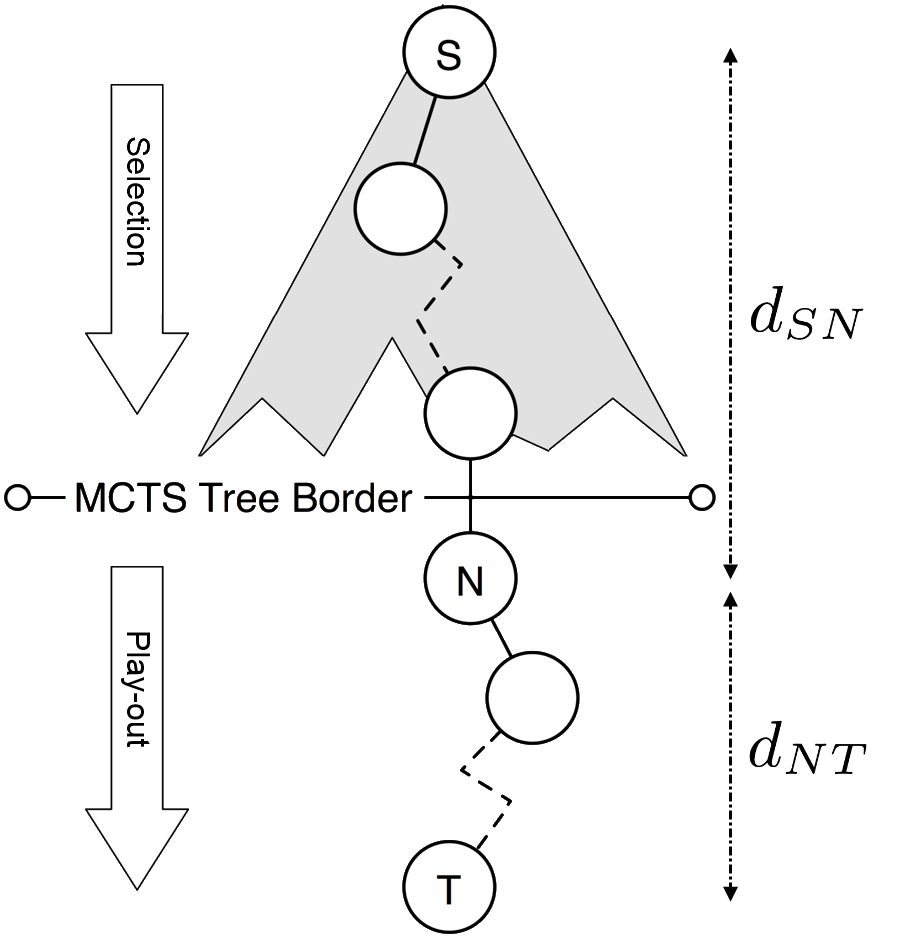
\includegraphics[width=.3\textwidth]{img/figure2_new.png}
	\caption{A single MCTS simulation \cite{finnsson2010learning}.}
	\label{fig:mcts-simulation}
\end{figure}
Moves played during play-out are selected by some play-out policy. Generally the play-out policy chooses moves at each state uniformly randomly, or is rule-based, reactive, or is combined with a source of expert or heuristic information such as an $\epsilon$-greedy policy \cite{sturtevant2008analysis, sutton1998reinforcement}. Various alternative methods have been proposed, such as using low-level $\alpha\beta$ searches \cite{Winands2011}, and methods that learn a strategy online, such and the Last-Good-Reply policy \cite{baier2010power}, Move-average Sampling Technique (MAST) \cite{finnsson2008simulation}, or using N-Grams \cite{Tak2012}. However, moves sampled from the play-out policy are far from optimal. Because numerous simulations are to be made during the time allowed for search, any play-out policy must be computationally efficient. Each move taken in the play-out step ultimately increases the uncertainty of the result obtained. Hence, the duration of the simulation may be regarded as an indicator of the certainty of the accuracy of the result.

The main benefit of using simulation duration as a quality measure is that it is domain independent. Unless the number of moves in the game is fixed, the duration of a simulation can be informative in determining its quality. In addition, simulation length has also previously been used to enhance the performance of the search~\cite{roschke2013cc,keller13thts}.

\subsection{Terminal State Quality}
\label{sub:termqual}
The second measure of a simulation's quality is based on a quality assessment of its specific terminal state reached. Evaluation functions can be designed for most games, they are used to evaluate non-terminal states and assign them a specific value. However, MCTS generally performs a play-out until a terminal state is reached. Therefore, we are interested in determining the quality of this terminal state directly to augment the information used by MCTS rather than the evaluation of an intermediary state. In some domains MCTS' performance is improved by using either a static, or an early cut-off of the simulations. In this paper, we do not consider these forms of quality assessment based on early cut-offs but rather we consider any extra information that can help describe the quality of a terminal state, such how convincing of a win it was for one side from in-game scores. 

As before, consider a single MCTS simulation as depicted in Figure \ref{fig:mcts-simulation}. When a terminal state is reached, a quality assessment function is called to evaluate the position with respect to the winning player. This measure $q$, should reflect the quality of a terminal state. For instance, in a game with material such as Breakthrough, Chess or Checkers, an evaluation can be based on scoring the remaining material of the winning player. For a racing game such as Chinese Checkers, the inverse of the number of pieces the opponent has in his target base can be considered. As such, the quality is based on the a posteriori evaluation of the terminal state. Having witnessed the states and actions performed from \node{S} to \node{T}, the score is based on an assessment of \node{T} given the progression \node{S} \ldots \node{N} \ldots \node{T} (see Figure \ref{fig:mcts-simulation}).

A similar quality bonus has previously been shown to enhance the performance of MCTS in BlokusDuo~\cite{shibahara2008combining}. Ours differs in that the quality bonus
is a function of its value compared to the mean quality value over all the play-outs.  

%-------------------------------------------------------------------
\section{QUALITY-BASED SIMULATION REWARDS}
\label{sec:qoreward}
This section discusses the foundation for altering MCTS play-out rewards. In Subsection \ref{sub:cv}, we describe control variates and explain how they can be used as a basis of the proposed quality measures discussed in the previous section. In Subsections \ref{subsec:rb} and \ref{subsec:qb}, \emph{Relative Bonus (RB)} and \emph{Qualitative Bonus (QB)} are defined, respectively. To conclude, in Subsection \ref{subsec:astar}, a method for determining an approximate value for $a$ is introduced, which is a constant used in the proposed methods.

In the proposed framework, MCTS simulations return a tuple of four reward values, $\tuple{r,\tau,q,d_{NT}}$ representing the outcome $r\in\{-1, 0, 1\}$, the winning player $\tau$, the quality assessment of the terminal state $q\in(0, 1)$, and the distance from the expanded node \node{N} to the terminal state \node{T}, $d_{NT}$, respectively. The distance $d\in(0, m)$, bounded above by the theoretical maximum duration of the game $m$, is then computed as shown in Equation \ref{eq:m_ST}. Apart from $q$, these values are available with minimal extra computational effort.

\subsection{Control Variates}
\label{sub:cv}
Variance reduction methods in mathematical simulation are used to improve estimates by reducing the variance in a simulation's output \cite{kelton2000simulation}. Recently, variance reduction techniques have been proposed for MCTS by Veness et al. \cite{Veness11variance}. They applied, among others, control variates to UCT in different stochastic games to improve results by the reducing variance of the estimators. However, their applications were mainly focused on reducing the variance that occurred from the stochastic domain. Furthermore, their control variates are recursively defined over sequences of states and actions. In this paper, we focus mainly on a simpler application of reducing the variance in the reward signal due to randomized play-outs.  

Control variates take advantage of a correlation between two random variables $X$ and $Y$, to improve estimators of $X$ given that the mean $v=\E{Y}$ is known. This is achieved by adding the deviation of $Y$ from its mean, scaled by a constant $a$, to $X$. We define a new random variable, 
\begin{equation}
Z=X+a\left(Y-v\right)
\label{eq:cv}
\end{equation}
and instead base estimates from observations of $Z$, which are based on paired observations $(X,Y)$, rather than just $X$ by itself. 
Here, $Y$ is called a {\it control variate} because its deviation from $\E{Y}$ is used to control the observed value $X$. 
One can show that there is a value $a^*=-\Cov{X,Y}\mathbin{/}\Var{Y}$ that minimizes $\Var{Z}$.

We define $X$ as the simulation outcome, i.e. $X_i=r$, and define $Y$ as as one of the quality measures discussed in Section \ref{sec:poqual}, $Y_i=d$ or $Y_i=q$. Then, assuming that $X$ and $Y$ are correlated, i.e. $\Corr{X,Y}\neq0$, we can compute an estimate of  $a^*$ from observations such that variance in the reward is reduced. In common practical domains, no fixed values for $v$, $\Cov{X,Y}$, or $\Var{Y}$ are known and appropriate estimators for these quantities are required.

\subsection{Relative Bonus}
\label{subsec:rb}
In this subsection, the Relative Bonus (RB) is introduced as an enhancement for the rewards generated by MCTS simulations. RB is based on the simulation duration discussed in Subsection \ref{sub:simdur} and used as a control variate as defined in the previous subsection.

First, note that $d$ depends on the domain, the progress of the game, and the play-out policy, and that the range of $d$ varies accordingly. Therefore, $d$ is standardized by defining it as a \emph{t}-statistic. A sample mean can be approximated online, by maintaining an average $\bar{D}^\tau$ for each player (indexed by $\tau$), over the distribution of observed $d$ values $D^\tau$. After each simulation, $\bar{D}^\tau$ is updated with the observed $d$, then $\hat{\sigma}^\tau_D$ is the sample standard deviation of the distribution $D^\tau$. Using these statistics, we define a standardized value $\lambda_r$ as follows:

\begin{equation}
\lambda_r = \frac{\bar{D}^\tau - d}{\hat{\sigma}^\tau_D}
\label{eq:rb_norm}
\end{equation}

Note that $\lambda_r$ is a function of $d$ but to simplify the notation we omit the dependency since it is always clear from the context. Also, $\lambda_r$ is both normalized with the sample standard deviation and is relative to $\bar{D}^\tau$. It is both independent of the progress of the game, and normalized with respect to the current variance in the length of simulations. When the number of samples is large, $\E{\lambda_r} \approx 0$ due to standardization and so $\lambda_r$ can be added to $r$ as a control variate with $v = 0$ in Eq.~\ref{eq:cv}. Note that, values of $\lambda_r$ are higher for shorter simulations.

Using an estimated mean may cause the search to be biased, i.e. moving into the direction of shorter games. Although there is no immediate solution to this problem, we propose to reset $\bar{D}^\tau$ and $\hat{\sigma}^\tau_D$ between moves. Moreover, rewards of the first $5\%$ of the expected number of simulations are not altered during search, and $\bar{D}^\tau$ and $\hat{\sigma}^\tau_D$ are updated during this time without altered selection.

Since the distribution of $D^\tau$ is not known, $\lambda_r$ can still take on unrestricted values, particularly if the distribution of $D^\tau$ is skewed, or has heavy tails on either side. Moreover, its relationship with the desired reward is not necessarily linear. As such, in order to both bound and shape the values of the bonus it is passed to a sigmoid function centered around $0$ on both axes whose range is $[-1,1]$,
\begin{equation}
b(\lambda)=-1+\frac{2}{1+e^{-k\lambda}}.
\label{eq:sigmoid}
\end{equation}
Here, $k$ is a constant to be determined by experimentation, it both slopes and bounds the bonus to be added to $r$. This type of function is commonly used to smooth reward values of evaluation functions. In \cite{shibahara2008combining}, $r$ was replaced by a sigmoid representing the final score.

Finally, the modified reward with the relative bonus is, 
\begin{equation}
r_b=r+\sgn(r) \cdot a \cdot b(\lambda_r).
\label{eq:rb}
\end{equation}
This value is backpropagated from the expanded leaf to the root node. The range of $r_b$ is $[-1-a, 1+a]$, i.e. the bonus $r_b$ is centered around the possible values of $r$. $a$ is either an empirically determined value, or computed off or on-line as described in Subsection \ref{subsec:astar}.

\subsection{Qualitative Bonus}
\label{subsec:qb}
The Qualitative Bonus follows the same procedure as the Relative Bonus. Similar to RB, the average $\bar{Q}^\tau$ and standard deviation $\hat{\sigma}^\tau_Q$ of observed $q$ values is maintained for each player $\tau$. The value of $q$ is determined by an assessment of the quality of the match's terminal state. Assuming that higher values of $q$ represent a higher quality terminal state for the winning player $\tau$, $\lambda_q$ is defined as:
\begin{equation}
\lambda_q = \frac{q - \bar{Q}^\tau}{\hat{\sigma}^\tau_Q}
\label{eq:qb_norm}
\end{equation}
Finally the bonus $b(\lambda_q)$ is computed using the sigmoid function in Equation \ref{eq:sigmoid} with an optimized $k$ constant, and summed with the result of the simulation $r$,
\begin{equation}
r_q=r+\sgn(r) \cdot a \cdot b(\lambda_q).
\label{eq:qb}
\end{equation}

\subsection{Estimating $a$}
\label{subsec:astar}
In gameplay, $X$ is a nominal variable, i.e. loss, draw, or win, and in our case, $Y$ is a discrete scalar. Therefore the method of determining $a^*$ is not straightforward. Moreover, since the quantities required to compute $a^*$, either online during search, or offline, are unknown for complex domains, $a^*$ can be an approximation at best. 
Efforts to determine a value for $a^*$ based on the intuitive definition of $X$ and $Y$, shown in Subsection \ref{sub:cv} did not result in practical values. Among others, determining the biserial covariance between $X$ and $Y$ was tried. However, due to the small covariance measured, the resulting range of $a^*$ was too small to make any impact on performance.

% (Tom) This was moved here from the first subsection
% (MarcL) I think this paragraph was too much in the wrong direction. Will say something smaller later.
%Although using the proposed quality measures as control variates is appropriate for MCTS, it is not necessarily the case that variance reduction results in performance increase. Therefore, although we expect that reducing the variance in the reward signal of MCTS is beneficial, it is not a guarantee. It is possible that a larger performance increase is gained by using a different value for $a$, as the quality measures may provide more advantage than variance reduction alone. Therefore, in this paper, we concentrate mainly on how these techniques can be used to improveme play performance. In conclusion, although we propose to define the quality-based rewards as control variates, in this paper we are not concerned with the actual reduction in variance, but rather the improvement in performance.

Nonetheless, a usable value for $a$, $a'$ can be computed and used online by using an alternative definition of $a^*$. As before, let $Y$ be either one of the proposed quality measured, i.e. $Y_i=d$ or $Y_i=q$, and let $\rho$ be the search player, i.e. the player running MCTS. Now separate $Y$ in another distinct random variable $Y^w$ such that
\begin{equation}
Y^w_i =
\begin{cases}
   Y_i & \text{if $w$ wins the play-out,} \\
   0   & \text{otherwise}
\end{cases}
\label{eq:ywin}
\end{equation}
Using this definition we can determine the sample covariance, $\SCov{Y^w,Y}$ in terms of $Y$ values only. This ensures there are no numerical differences between the quantities. Next, we can compute 
\begin{equation}
	a'=\left|{\SCov{Y^w,Y}}\mathbin{/}{\SVar{Y}}\right|
\label{eq:onlinea}
\end{equation}
and use it, as the value for $a$ in Equations \ref{eq:rb} and \ref{eq:qb}. 

Because the choice of $Y^w$ is arbitrary, since every game is won by either one of the players, the actual value of $a'$ is treated as a magnitude, and its sign is not used. This works because the assumption is made that 1) shorter games are preferred over long ones (Equation \ref{eq:rb_norm}) and, 2) higher $q$ values indicate better play-out quality (Equation \ref{eq:qb_norm}).

%-------------------------------------------------------------------
\section{PSEUDO-CODE}
Algorithm~\ref{alg} summarizes a single iteration of MCTS enhanced with RB or QB. Note that negamax backups are used in this setup, and therefore $r$ is relative to the player to move at the node that initiates the play-out. The basic MCTS algorithm used in this paper is the MCTS-Solver \cite{Winands2008}, although the details of its implementation are omitted in the pseudo-code. Whenever \emph{update} is used in the algorithm, it refers to updating the average reward for a node, or the sample mean and standard deviation for $\bar{D}^\tau$ and $\bar{Q}^\tau$.

\begin{algorithm2e}[ht]
\setstretch{1.07}
  {\sc mcts}(node $p$, node depth $d_{Sp}$):														\;
  \pushline
    \lIf{isLeaf($p$)}{Expand($p$)}
    Select a child $i$ according to Eq.~\ref{eq:uct} 												\;
    $d_{Si} \gets d_{Sp} + 1$																		\; \label{alg:depth}
    \eIf{$n_i = 0$}{
    	$\tuple{r, \tau, q, d_{iT}} \gets$ {\sc playout}$(i)$ 											\; \label{alg:results}
    	$d \gets d_{Si} + d_{iT}$																	\;			
    	\If{enabled$(b_r)$ and $\hat{\sigma}^\tau_D > 0$}{
    		$r \gets r + \sgn(r) \cdot a~\cdot $ {\sc bonus}$(\bar{D}^\tau - d, \hat{\sigma}^\tau_D)$ 	\; \label{alg:rb}
    		update $\bar{D}^\tau$ and $\hat{\sigma}^\tau_D$ with $d$								\; 		\label{alg:meanstddev}
		  }
  		\If{enabled$(b_q)$ and $\hat{\sigma}^\tau_Q > 0$} {
    		$r \gets r + \sgn(r) \cdot a~\cdot $ {\sc bonus}$(q -\bar{Q}^\tau, \hat{\sigma}^\tau_Q)$ 	\; \label{alg:qb}
    		update $\bar{Q^\tau}$ and $\hat{\sigma}^\tau_Q$ with $q$ 								\;
    	}
    	update node $i$ with $r$																	\;
    }{
    	$r \gets$ -{\sc mcts}($i$, $d_{Si}$)														\; 
    }
    update node $p$ with $r$																		\;
   \popline
    {\bf return} $r$																				\;
  																									\;
    {\sc bonus}(offset from mean $\delta$, sample std. dev. $\hat{\sigma}$):						\;	\label{alg:bonus}
    \pushline
    	$\lambda \gets \nicefrac{\delta}{\hat{\sigma}}$												\;	\label{alg:lambda}
    	$b \gets -1+\nicefrac{2}{\left(1+e^{-k\lambda}\right)}$										\;	\label{alg:b}
    \popline
    \bf{return} $b$																					\;
  \vspace{0.3cm}
  \caption{Pseudo-code of quality-based MCTS (Section \ref{sec:qoreward}). \label{alg}}
\end{algorithm2e}

During selection, starting from the root, the depth of the current node is updated on line \ref{alg:depth}. Whenever an expandable node is reached, its children are added to the tree and a play-out is initiated from one of them. A play-out returns a tuple of results, on line \ref{alg:results} four different values are returned: 1) the result of the play-out $r \in \{-1, 0, 1\}$, 2) the winning player $\tau$, 3) the assessed quality of the play-out's terminal state $q\in(0,1)$, and 4) the number of moves made during play-out $d_{iT}$ defined in Subsection~\ref{sub:simdur}. Using these values $r$ is altered. On line \ref{alg:rb} the relative bonus is applied to $r$, using the difference with the winning player's current mean $\bar{D}^\tau - d$, i.e. lower values of $d$ give a higher reward. After which the current mean and standard deviation are updated on line \ref{alg:meanstddev}. QB is applied on line \ref{alg:qb} using the assessed quality of the play-out $q$. Note that the offset from the mean is defined as $q - \bar{Q}^\tau$, because in contrast to RB, positive deviation of $q$ from its mean imply better results. The {\sc bonus} function on line \ref{alg:bonus}, computes the normalized $\lambda$ (line \ref{alg:lambda}) and, successively the bonus $b$ (line \ref{alg:b}) using the sigmoid function, as defined in Subsections \ref{subsec:rb} and \ref{subsec:qb}. The constant $a$ on lines \ref{alg:rb} and \ref{alg:qb} can be either fixed, or computed online as shown in Subsection \ref{subsec:astar}.

%-------------------------------------------------------------------
\section{EXPERIMENTS}
\label{sec:experiments}
To determine the impact on performance of RB and QB, experiments were run on six different two-player games. Moreover, the performance of RB is evaluated in the General Game-playing agent {\sc CadiaPlayer} \cite{bjornsson2009cadiaplayer}, which won the International GGP competition in 2007, 2008, and 2012.

\subsection{Experimental Setup}
\label{subsec:expsetup}
The proposed enhancements are validated in six distinct two-player games. These games are implemented to use a single, uniform implementation of MCTS.
\begin{itemize}
\item \emph{Amazons} is played on a 10$\times$10 chessboard. Each player has four amazons that move (and shoot) as queens in chess. However, each move consist of two parts, first the amazon moves, after which she must fire an arrow on an empty position in range, and this square on the board is blocked. The last player to move wins the game.
\item \emph{Breakthrough} is played on an 8$\times$8 board. Each player starts with 16 pawns on one side of the board and the aim is to move one of them to the opposite side.
\item \emph{Cannon} is a chess-like game where the goal is to checkmate your opponent's immobile town. Each player has one town he must place at the start of the game, and 15 soldiers. Soldiers can move or capture forward or may retreat if next to an opponent's soldier. Moreover, three soldiers in a row form a cannon that can move and shoot across the board.
\item \emph{Checkers} is played on an 8$\times$8 board, and the goal is to capture all opponent's pieces.
\item \emph{Chinese Checkers} is played on a star-shaped board. Each player starts with six pieces placed in one of the star's points, and the aim is to move all six pieces to the opposite side of the board. This is a variation of the original Chinese Checkers which is played on a larger board with 10 pieces per player.
\item \emph{Pentalath} is a connection game played on a hexagonal board. The goal is to place 5 pieces in a row. Pieces can be captured by fully surrounding an opponent's set of pieces.
\end{itemize}

The following values of $q$ are used for each game. \emph{Amazons}: the combined number of moves available for the winning player. \emph{Breakthrough} and \emph{Cannon}: the total piece difference between the winning and losing player. \emph{Checkers}: the total number of pieces in play for the winning player. \emph{Chinese Checkers}: the inverse number of the losing player's pieces that reached the home-base. \emph{Pentalath}: the inverse of the longest row of the losing player, given that this row can be extended to a length of 5.
For each quality measure an appropriate, fixed, normalizer brings the measure within the $[0,1]$ range. 

For each game, an appropriate play-out policy is used to select moves to make during play-out. They are implemented to ensure that no obvious mistakes or flawed play is observed. All results are reported with these play-out policies enabled.

GGP experiments are performed using the {\sc CadiaPlayer} code base. In GGP, no domain knowledge is available in advance, rules of the games are interpreted online resulting in low simulation counts. Moreover, play-out policies are learned online, using N-Grams \cite{takngrams}. The following two-player turn-based games were used to analyze the performance of the enhancement: Zhadu, TTCC4, Skirmish, SheepWolf, Quad, Merrils, Knightthrough, Connect5, Checkers, Breakthrough, 3DTicTacToe and Chinese Checkers. We show results for two simultaneous move games: Battle and Chinook.

Experiments were run on 2.2Ghz AMD Opteron CPU running 64-bit Linux 2.6.18. For each game, the constant $k$ used by the sigmoid function was determined by experimenting with values between 0 and 10, with varying increments. The $C$ constant, used by UCT (Equation \ref{eq:uct}) was optimized or each game without any enhancements enabled and was not altered nor re-optimized for the experiments.
\subsection{Results}
\label{subsec:results}
For each result, the winning percentage is reported for the player with the enhancement enabled, along with a 95\% confidence interval. For each experiment, the players' seats were swapped such that 50\% of the games are played as the first player, and 50\% as the second, to ensure no first-player or second-player bias.

\begin{table}
{\caption{Relative Bonus enabled using different search times, 5000 games} \label{tab:rb}}
\begin{center}
\tabcolsep=0.15cm
\scalebox{0.93}{
\begin{tabular}{rlrrrr}
\hline
\multicolumn{2}{r}{\rule{0pt}{12pt}\textbf{Search time}} & \multicolumn{2}{c}{\textbf{1 second}} & \multicolumn{2}{c}{\textbf{5 seconds}} \\
\cline{1-6}
\rule{0pt}{12pt}
\textbf{Game} & \multicolumn{1}{c|}{\textbf{$k$}} 
& \multicolumn{1}{c}{\textbf{$a'$}} & \multicolumn{1}{c}{\textbf{$a = 0.25$}} & \multicolumn{1}{c}{\textbf{$a'$}} & \multicolumn{1}{c}{\textbf{$a = 0.25$}} \\ \hline
Amazons &\multicolumn{1}{l|}{2.2}			    & {\bf{54.7}} $\pm$ 1.4 		& {\bf{55.7}} $\pm$ 1.4 		& {\bf{54.8}} $\pm$ 1.4	 & {\bf{54.7}} $\pm$ 1.4 	\\ 
Breakthrough &\multicolumn{1}{l|}{8.0} 			& 50.0 $\pm$ 1.4		    	& 51.0 $\pm$ 1.4 		    	& 47.6 $\pm$ 1.4			   & {\bf{51.6}} $\pm$ 1.4 	\\ 
Cannon &\multicolumn{1}{l|}{3.0} 			    & {\bf{62.8}} $\pm$ 1.3 		& {\bf{60.6}} $\pm$ 1.3 		& {\bf{58.8}} $\pm$ 1.4 & {\bf{58.1}} $\pm$ 1.4 	\\ 
Checkers &\multicolumn{1}{l|}{2.8}			  	& {\bf{52.1}} $\pm$ 0.8 		& {\bf{52.7}} $\pm$ 0.8 		& 48.9 $\pm$ 0.7	 & {\bf{50.7}} $\pm$ 0.6 	\\ 
Chin. Checkers &\multicolumn{1}{l|}{1.2} 		& {\bf{56.8}} $\pm$ 1.4 		& {\bf{53.2}} $\pm$ 1.4 		& {\bf{54.9}} $\pm$ 1.4	 & {\bf{52.5}} $\pm$ 1.4 	\\
Pentalath &\multicolumn{1}{l|}{1.0} 		  	& {\bf{51.4}} $\pm$ 1.4 		& 50.3 $\pm$ 1.4 		      	& 49.3 $\pm$ 1.4 		     & 49.5 $\pm$ 1.4 		\\
\hline
\end{tabular}
}
\end{center}
\end{table}
Results for relative bonus are shown in Table \ref{tab:rb}. When using one second of search time, a significant increase in performance is shown for five of the six games, and no adverse results in the other. The value of $k$ was optimized empirically once for each game, and all experiments use the reported value in the second column. 
We try a fixed value of $a = 0.25$ in addition to online definition of $a'$ from Eq.~\ref{eq:onlinea}. We see that the online $a'$ leads to increased performance over a fixed value for five games. 
Interestingly, at five seconds of search time, a fixed value tends to lead to more consistent results over the five games. 
In Breakthrough, %, defense is equally important as offense, 
and since the play-out policy does not contain heuristics for complicated defensive positioning, the play-outs' lengths favors quick wins and exclude defensive moves.
Chinese Checkers, Cannon and Amazons achieve the most increase in performance using RB. These games improve the estimates of their length over time, and penalizing long games at the beginning of the match could ensures better estimates since the length of the actual match is shorter overall. Pentalath is a game with a limited length, when the board is nearly filled the game is sure to end. As such, the additional information provided by the length of games is limited.
\begin{table}
{\caption{Relative Bonus in GGP, {\sc{CadiaPlayer}}, $a = 0.25$ \newline 30 sec. startclock, 15 sec. playclock} \label{tab:rb_ggp}}
\begin{center}
\tabcolsep=0.25cm
\scalebox{0.93}{
\begin{tabular}{rrr}
\hline
& \multicolumn{1}{c}{\textbf{$k = 2$}} & \multicolumn{1}{c}{\textbf{$k = 1.4$}} \\
\cline{1-3}
\multicolumn{1}{c|}{\rule{0pt}{12pt}\textbf{Game}} & \multicolumn{1}{c}{\textbf{$a = 0.25$}} & \multicolumn{1}{c}{\textbf{$a = 0.25$}} \\ \hline
\multicolumn{1}{r|}{Zhadu} 			  	&{\bf{54.3}} $\pm$ 1.9			& {\bf{53.3}} $\pm$ 1.9 	\\
\multicolumn{1}{r|}{TTCC4} 				&{\bf{55.3}} $\pm$ 2.0			& {\bf{53.3}} $\pm$ 2.0 	\\
\multicolumn{1}{r|}{Skirmish} 			&51.9 $\pm$ 2.2		    		& 50.7 $\pm$ 2.2 			\\
\multicolumn{1}{r|}{SheepWolf} 			&51.7 $\pm$ 1.9   				& {\bf{52.3}} $\pm$ 1.9 	\\
\multicolumn{1}{r|}{Quad} 				&{\bf{44.7}} $\pm$ 1.8			& {\bf{44.7}} $\pm$ 1.8 	\\
\multicolumn{1}{r|}{Merrills} 			&51.9 $\pm$ 2.6		    		& 48.9 $\pm$ 2.6 			\\
\multicolumn{1}{r|}{Knightthrough}		&49.9 $\pm$ 2.1   				& 49.2 $\pm$ 2.1 			\\
\multicolumn{1}{r|}{Connect5} 			&{\bf{54.0}} $\pm$ 1.8			& {\bf{54.4}} $\pm$ 1.8 	\\
\multicolumn{1}{r|}{Checkers} 			&{\bf{54.4}} $\pm$ 3.0			& 52.1 $\pm$ 3.2 			\\
\multicolumn{1}{r|}{Breakthrough}		&51.3 $\pm$ 2.9			    	& 51.0 $\pm$ 2.9 			\\
\multicolumn{1}{r|}{3DTicTacToe}		&{\bf{55.0}} $\pm$ 1.6			& {\bf{54.5}} $\pm$ 1.6 	\\
\multicolumn{1}{r|}{Chin. Checkers}		&{\bf{56.3}} $\pm$ 1.8			& {\bf{56.0}} $\pm$ 1.8 	\\
\hline
\multicolumn{1}{r|}{Battle}				&50.0 $\pm$ 2.0	    			& 49.2 $\pm$ 2.0 			\\
\multicolumn{1}{r|}{Chinook} 			&48.5 $\pm$ 2.0	    			& 49.0 $\pm$ 2.0 			\\
\hline
\end{tabular}
}
\end{center}
\end{table}

For the GGP domains, results are presented in Table \ref{tab:rb_ggp}. A single value for $a$ was used for GGP because a significant number of simulations are required to compute an accurate $a'$. Moreover, since values for $k$ can not be optimized beforehand, we present the results for two different $k$ values. Although $k$ has an influence on the performance of RB, it is robust with respect to suboptimal values, and an approximation can be used as is made clear by the results in Table \ref{tab:rb_ggp}. All games that benefit from RB does so for either both values, or it is not disadvantageous for either value. Note that the results for Chinese Checkers, Checkers and Breakthrough are similar to those in Table \ref{tab:rb}, demonstrating the robustness of the enhancement. Regarding both Tables \ref{tab:rb} and \ref{tab:rb_ggp}, we have demonstrated that the results are invariant with respect to the number of simulations per move.

\begin{table}
{\caption{Qualitative Bonus using different search times, 5000 games} \label{tab:qb}}
\tabcolsep=0.15cm
\begin{center}
\scalebox{0.93}{
\begin{tabular}{rlrrrr}
\hline
\multicolumn{2}{r}{\rule{0pt}{12pt}\textbf{Search time}} & \multicolumn{2}{c}{\textbf{1 second}} & \multicolumn{2}{c}{\textbf{5 seconds}} \\
\cline{1-6}
\rule{0pt}{12pt} \textbf{Game} & \multicolumn{1}{c|}{\textbf{$k$}} 
& \multicolumn{1}{c}{\textbf{$a'$}} & \multicolumn{1}{c}{\textbf{$a = 0.25$}} & \multicolumn{1}{c}{\textbf{$a'$}} & \multicolumn{1}{c}{\textbf{$a = 0.25$}} \\ \hline
Amazons &\multicolumn{1}{l|}{1.6}			    & {\bf{64.5}} $\pm$ 1.3 & {\bf{58.0}} $\pm$ 1.4 	& {\bf{63.0}} $\pm$ 1.3 	& {\bf{57.7}} $\pm$ 1.4 \\
Breakthrough &\multicolumn{1}{l|}{2.0} 		& {\bf{74.8}} $\pm$ 1.2 & {\bf{71.9}} $\pm$ 1.2 	& {\bf{76.3}} $\pm$ 1.2 	& {\bf{78.6}} $\pm$ 1.1 \\
Cannon &\multicolumn{1}{l|}{4.0} 			    & {\bf{65.9}} $\pm$ 1.3 & {\bf{63.0}} $\pm$ 1.3 	& {\bf{54.7}} $\pm$ 1.4 	& {\bf{57.4}} $\pm$ 1.4 \\
Checkers &\multicolumn{1}{l|}{2.0}			  & {\bf{53.8}} $\pm$ 0.8 & {\bf{52.7}} $\pm$ 0.7 	& {\bf{51.9}} $\pm$ 0.6 	& {\bf{52.3}} $\pm$ 0.6 \\
Chin. Checkers &\multicolumn{1}{l|}{2.8} 	& {\bf{65.7}} $\pm$ 1.3 & {\bf{60.1}} $\pm$ 1.4 	& {\bf{61.4}} $\pm$ 1.3 	& {\bf{58.9}} $\pm$ 1.4 \\
Pentalath &\multicolumn{1}{l|}{1.6} 		  & 46.6 $\pm$ 1.4  	     & 50.5 $\pm$ 1.4 		    & 48.7 $\pm$ 1.4		 	    & 50.1 $\pm$ 1.4 \\
\hline
\end{tabular}
}
\end{center}
\end{table}

Results for QB are shown in Table \ref{tab:qb}. A significant increase in performance is presented for five of the six games. The quality assessment in Pentalath is expensive and not very informative as the longest row of the opponent is not likely to make a difference in winning the game. All other games use simple assessments of their terminal states, which required little to no added computational effort. In the case of Breakthrough and Cannon, which show the highest overall performance increase, the quality assessments are not directly related to winning the game. As is the case with RB, the results are invariant with respect to the number of simulations per move.

\begin{table}
{\caption{Qualitative Bonus and Relative Bonus combined using different search times, 5000 games} \label{tab:qbrb}}
\tabcolsep=0.15cm
\begin{center}
\scalebox{0.93}{
\begin{tabular}{rrrrr}
\hline
\multicolumn{1}{r}{\rule{0pt}{12pt}\textbf{Search time}} & \multicolumn{2}{c}{\textbf{1 second}} & \multicolumn{2}{c}{\textbf{5 seconds}} \\
\cline{1-5}
\rule{0pt}{12pt} \textbf{Game} & \multicolumn{1}{c}{\textbf{$a'$}} & \multicolumn{1}{c}{\textbf{$a = 0.25$}} & \multicolumn{1}{c}{\textbf{$a'$}} & \multicolumn{1}{c}{\textbf{$a = 0.25$}} \\ \hline
Amazons 		& $\pm$  & {\bf{61.9}} $\pm$ 1.4	& $\pm$  & {{\bf60.9}} $\pm$ 1.4	\\
Breakthrough 	& $\pm$  & {\bf{72.9}} $\pm$ 1.2	& $\pm$  & {{\bf78.6}} $\pm$ 1.1 	\\
Cannon 			& $\pm$  & {\bf{69.3}} $\pm$ 1.3 	& $\pm$  & {{\bf62.3}} $\pm$ 1.3 	\\
Checkers 		& $\pm$  & {\bf{54.1}} $\pm$ 0.8 	& $\pm$  & {{\bf53.5}} $\pm$ 0.7	\\
Chin. Checkers 	& $\pm$  & {\bf{63.1}} $\pm$ 1.3  	& $\pm$  & {{\bf70.0}} $\pm$ 1.4	\\
Pentalath 		& $\pm$  & 51.2 $\pm$ 1.4  			& $\pm$  & {{\bf51.4}} $\pm$ 1.4 	\\
\hline
\end{tabular}
}
\end{center}
\end{table}

Note that while the gains are higher for QB, RB does not require any domain knowledge. An immediate question is 
whether the two methods are complementary. Results with both methods enabled are shown in Table~\ref{tab:qbrb}. 
Comparing to Tables~\ref{tab:rb} and \ref{tab:qb}, in $X$ of the $Y$ cases the gain for 
the combination is higher than each bonus on its own.

%-------------------------------------------------------------------
\section{CONCLUSION}
\label{sec:concl}
%Limited work has been done to improve the reward signal used to approximate positions in Monte-Carlo Tree Search (MCTS). 
In this paper, we show that the performance of MCTS is improved by treating the rewards of simulations as a combination of the win/loss state, with a quality measure. The enhancements are implemented using control variates, a well-known variance reduction technique. We show performance can be improved when there is a non-zero correlation between the reward-signal and the quality measure. This was true for both bonuses in most of the game domains we used. 
%The experimental results show that using an additional informative statistic as a control variate in MCTS' results will improve overall performance in most domains.

The Relative Bonus (RB) treats the length of a simulation as a measure of its quality. The benefit of this method is that it is domain-independent. It seems to perform best in games where there is high variance in play-out lengths, favoring the shorter ones. 
%When the length of simulations is close to the length of the match played, RB provides less added information, and therefore only minor performance enhancements. 
%RB is especially interesting for General Game-Playing (GGP), where knowledge of the games played is sparse. 
In General Game-Playing, RB improved empirical performance in 14 of the 24 sequential game cases, and did not significantly decrease performance in any of the cases. 
The Quality Bonus (QB) improved results in all (non-GGP) domains, though its implementation requires additional knowledge. Nonetheless, even simple quality assessments of terminal states, such as a piece count, improves results considerably.

%We considered only cases where play-outs reach a natural end-state. 
For some domains this is not feasible or practical for play-outs to reach a natural terminal state. Therefore, we propose combining early and static cut-offs of play-outs as future research. Although a static cut-off will not be compatible with RB, we expect both to improve performance in combination with QB. Moreover, combining RB and QB with the reward signal may be improved by computing the $a'$ from the covariance matrix as is standard when combining control variates. 
%between the simulation's reward signal, the simulation's duration, and quality assessment, and computing separate scaling constants for each.
Finally, we hope that the proposed enhancements could improve estimates of online learning methods for play-out policies such as n-grams, or MAST. % though this is left for future research.

%-------------------------------------------------------------------
%\ack This work is partially funded by Scientific Research (NWO) in the framework of the project Go4Nature, grant number 612.000.938, and in the framework of the project GoGeneral, with grant number 612.001.121.

\bibliography{references}

\end{document}
